\documentclass{article}
\usepackage{graphicx} % Required for inserting images

\title{Labwork 3 Advanced Programming for HPC}
\author{Ta Quang Hieu - M22ICT002}
\date{October 2023}

\begin{document}
	
	\maketitle
	
	\section{The problem}
	Labwork 3: Threads
	\begin{enumerate}
		\item Copy labwork 3 code to labwork 4
		\item Improve labwork 4 code to use 2D blocks
		\item Use time.time() to measure speedup
	\end{enumerate}
	
	Figure ~\ref{fig:python} the image that I used in this labwork:
	
	\begin{figure}
		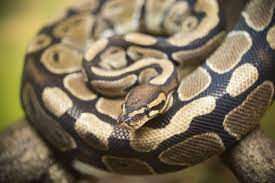
\includegraphics[width=\linewidth]{python.jpg}
		\caption{A python in rgb.}
		\label{fig:python}
	\end{figure}
	
	\section{Using GPU - with 1D block and grid}
	This is the kernel that I had used to convert an image to grayscale using GPU - 1d:
	\begin{verbatim}
		# Define a Numba CUDA kernel for grayscale conversion
		@cuda.jit
		def grayscale(src, dst):
		# where are we in the input?
		tidx = cuda.threadIdx.x + cuda.blockIdx.x * cuda.blockDim.x
		g = np.uint8((src[tidx, 0] + src[tidx, 1] + src[tidx, 2]) / 3)
		dst[tidx, 0] = dst[tidx, 1] = dst[tidx, 2] = g
	\end{verbatim}
	The part \textbf{@cuda.jit} shows that this is a kernel that will be executed by the GPU. And basically what it does it just like the previous part in CPU, where we take the average of the channels. Below is the script to convert to grayscale using GPU with the running time of \textbf{0.1298370361328125} seconds:
	
	\begin{verbatim}
		# Define a Numba CUDA kernel for grayscale conversion
		@cuda.jit
		def grayscale(src, dst):
		# where are we in the input?
		tidx = cuda.threadIdx.x + cuda.blockIdx.x * cuda.blockDim.x
		g = np.uint8((src[tidx, 0] + src[tidx, 1] + src[tidx, 2]) / 3)
		dst[tidx, 0] = dst[tidx, 1] = dst[tidx, 2] = g
	\end{verbatim}
	
	Figure ~\ref{fig:gpu_python} is the result produced by GPU:
	
	\begin{figure}
		\includegraphics[width=\linewidth]{gpu_python_1d.png}
		\caption{A grayscale python - using gpu.}
		\label{fig:gpu_python}
	\end{figure}
	
	\subsection{Block size vs time}
	This is the result that I take block size from 2\^1 to 2\^9:
	\begin{verbatim}
		[0.08243799209594727,
		0.0013549327850341797,
		0.0007569789886474609,
		0.0008955001831054688,
		0.0006525516510009766,
		0.0006351470947265625,
		0.0006105899810791016,
		0.0006227493286132812,
		0.0008649826049804688]
	\end{verbatim}
	Which will turn to a plot like in Figure ~\ref{fig:plot}:
	\begin{figure}
		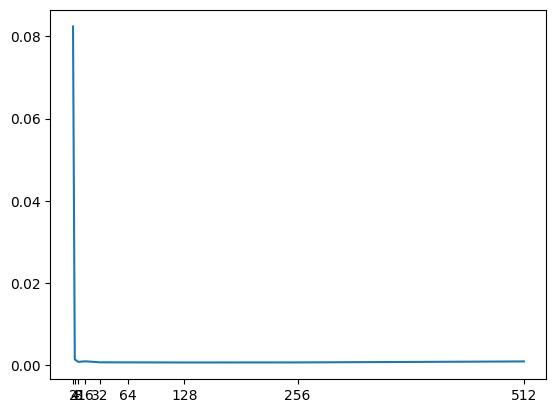
\includegraphics[width=\linewidth]{plot.png}
		\caption{A grayscale python - using gpu.}
		\label{fig:plot}
	\end{figure}
	
	\section{Using GPU - with 2D block and gird}
	This is the script that I had used to convert an image from RGB to grayscale. Basically, I create a new grayscale image by take the average from the red, green and blue channel. The running time using GPU is \textbf{0.00092315673828125} seconds for block size of 32*32.
	\begin{verbatim}
		# Define a Numba CUDA kernel for grayscale conversion
		@cuda.jit
		def grayscale(src, dst):
		# where are we in the input?
		tidx = cuda.threadIdx.x + cuda.blockIdx.x * cuda.blockDim.x
		tidy = cuda.threadIdx.y + cuda.blockIdx.y * cuda.blockDim.y
		
		g = np.uint8((src[tidx, tidy, 0] + src[tidx, tidy, 1] + src[tidx, tidy, 2]) / 3)
		dst[tidx, tidy, 0] = dst[tidx, tidy, 1] = dst[tidx, tidy, 2] = g
	\end{verbatim}
	
	About grid size, It must be rectangular, else the image will be cropped for some pixels.
	
	Figure ~\ref{fig:cpu_python} is the result produced by GPU:
	
	\begin{figure}
		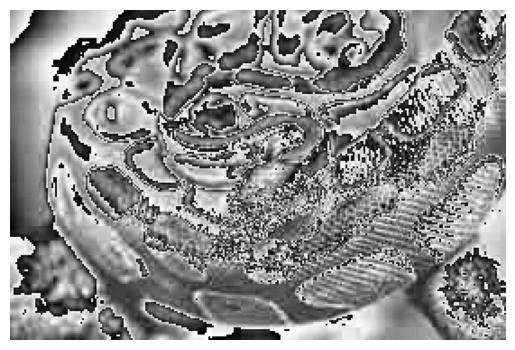
\includegraphics[width=\linewidth]{cpu_python.png}
		\caption{A grayscale python - using gpu.}
		\label{fig:cpu_python}
	\end{figure}
	
	\subsection{Block size vs time}
	This is the result that I take block size from 2\^1 to 2\^5:
	\begin{verbatim}
		[0.00241851806640625,
		0.0010306835174560547,
		0.0011587142944335938,
		0.0010194778442382812,
		0.00092315673828125]
	\end{verbatim}
	Which will turn into a plot like in Figure ~\ref{fig:plot_2d}:
	\begin{figure}
		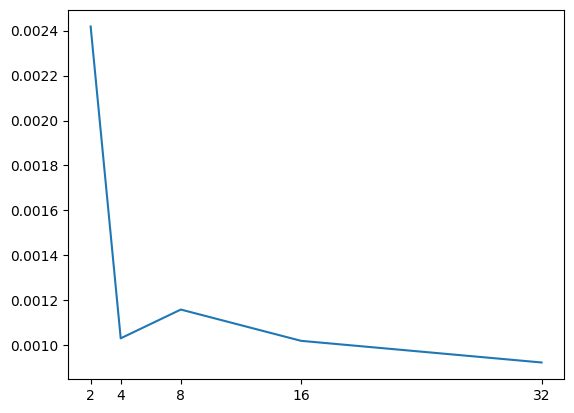
\includegraphics[width=\linewidth]{plot_2d.png}
		\caption{A grayscale python - using GPU - 2d grid and block.}
		\label{fig:plot_2d}
	\end{figure}
	
	I can only run to 32*32 block size with 2d, and as we can observe using 2bd block size makes the program run faster.
	
\end{document}
